\documentclass{article}
\usepackage{graphicx}
\usepackage{amsmath}
\usepackage[table]{xcolor}

\begin{document}
\newcommand{\vect}[1]{\mathbf{#1}}

\title{Ionic Liquid Propellant Burn Rate Model using Bayesian Inversion}
\author{Brandon Denton}
\date{Sept. 28, 2017}

\maketitle

\section{Introduction} \label{intro}

A current development area for next generation monopropellant rockets is technology related to the use of
ionic liquid monopropellants. These next generation monopropellants have the potential of providing greater
than 50% increase in specific impulse (Isp) over current state-of-the-art hydrazine thrusters. 
A consequence of this performance increase is much higher combustion temperatures resulting in material 
strength concerns. In addition to the increase in combustion temperature, these propellants can show dramatic
changes in burn rate in different pressures regimes often showing an inflection point where the burn rate goes
high order. Understanding the chemical mechanisms responsible for these characteristics will enable optimal thruster 
designs based on these monopropellants.

The work presented in this report uses Bayesian Inversion Methods and burn rate data of a candidate ionic liquid 
propellant from Strand burner testing at different pressures to determine the pre-exponential coefficient ($A$) and 
pressure exponential ($n$) of Saint Robert's Law as well as its uncertainty. The Bayesian Inversion analysis was performed 
by utilizing the Quantification of Uncertainty for Estimation, Simulation and Optimization (QUESO) code developed by E. 
Prudencia \& K. Schulz with additional contributions from the software community.

\section{Background} \label{background}

A short discussion on the relevant background information for Saint Robert's Law and the Strand burner testing is 
provided below for completeness. These subjects are not the primary interest of this report and as such additional 
details on either of these subjects are left for the reader to independently investigate.

\subsection{Saint Robert's Law} \label{St_Roberts_Law}

Saint Robert's Law is a power law relationship between pressure and propellant burn rate and is stated as:
\begin{equation}
R_b=A \cdot P^n
\end{equation}

It is often used to describe the burn rates of solid rocket propellants. However, it has been successfully 
adopted to describe the relationship between burn rate and pressure for liquid propellants. The analysis 
presented in this report assumes that this relationship holds for the candidate ionic liquid propellant investigated. 


\subsection{Strand Burner \& Apparatus Testing} \label{Apparatus_Test}

A Strand Burner is a constant volume optical pressure vessel which allows for the observation and measurement of 
propellant burn rates at different pressures. The propellant of interest is placed in a transparent borosilicate 
cylindrical tube within the strand burner, subjected to controlled constant pressure created with non-reacting 
gaseous nitrogen and ignited via a resistively heated nichrome wire and small quantity of double-base propellant. 
The propagation of the flame front as it consumes the propellant is recorded via a digital camera and the average 
burn rate is calculated post-test by averaging multiple measurements for the same test based on recording time stamps 
and visual measurements. Figure \ref{fig1} shows a schematic and actual photograph of the Strand burner used to collect 
the data presented as part of this report. Figure \ref{fig2} shows an example of a series of images captured during a test 
and from which the average burn rate for the test is calculated.

\begin{figure}[htb]
\centering
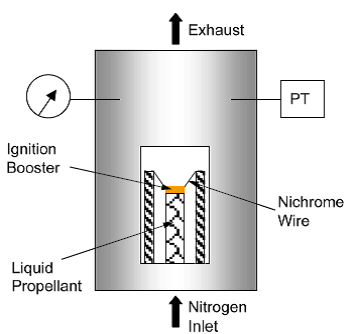
\includegraphics[width=0.48\textwidth]{Strand_Burner_image_1.png}
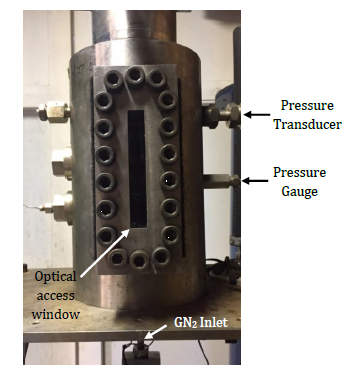
\includegraphics[width=0.48\textwidth]{Strand_Burner_image_2.png}
\caption{Strand Burner Schematic \& Image}
\label{fig1}
\end{figure}

\begin{figure}[htb]
\centering
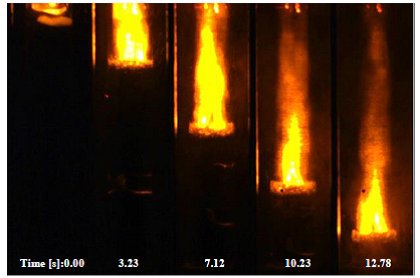
\includegraphics[width=0.48\textwidth]{Burn_Time_Elapse.png}
\caption{Series of Images Captured during a Single Test}
\label{fig2}
\end{figure}

Multiple tests at various pressures were conducted. Tests with different diameter cylindrical tubes between 10 mm to
16 mm were also conducted. Comparisons of burn rate observations between different diameter cylindrical tubes at the
same pressure showed that the diameter of the tube had little effect on the burn rate. The burn rates observed during 
these tests are presented in Figure \ref{fig3}. The figure also shows the curve fit results generated using linear regression 
via frequentist methods by the experimenters. The error bars shown is the calculated error for each individual test. A 
comparison of these parameters against the ones inferred in this report using Bayesian Inversion Methods will be of 
interest and are discussed later. One last note about the results is the apparent self-quenching of the propellant when 
the pressure is between 650 psia and 780 psia. This behavior was not expected and is currently unexplained. An analysis 
of the combustion kinetics of this propellant may provide some insight into this behavior. However, at the time of this 
report�s writing, the system of combustion reactions for this propellant is not well characterized or understood. Research 
in this area is currently being undertaken.

\begin{figure}[htb]
\centering
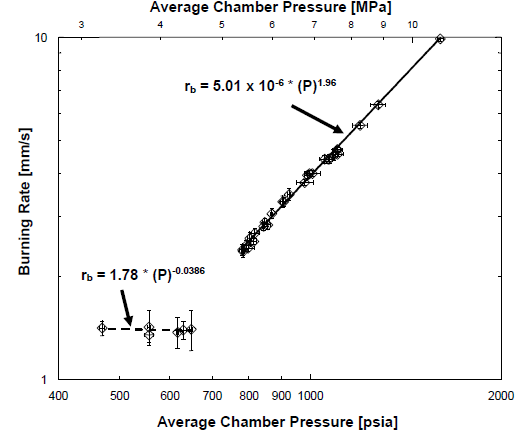
\includegraphics[width=0.75\textwidth]{Experimentors_Obs_fit.png}
\caption{Observed Burn Rates for Candidate Ionic Liquid Propellant}
\label{fig3}
\end{figure}

\section{Bayesian Inversion Analysis} \label{Bayesian_Inv_Analysis}

Bayesian Inversion methods were employed with the objectives of determining 1) the maximum likelihood estimation for
the pre-exponential coefficient A and exponential n of Saint Robert�s burn rate law and 2) the 95\% confidence interval 
of the model for the pressure range of interest given the data. The following sections detail the theoretical 
underpinnings utilized for the analysis of the data presented in Section \ref{Apparatus_Test} as well as the setup of QUESO.

\subsection{Theoretical Development} \label{Theory_Dev}

Theoretical development of the model was accomplished by assuming that the burn rate data is independent and 
identically distributed, the likelihood probability density function of the burn rate is Gaussian, the prior 
is uniform and the error is additive (Eq. \ref{add_err}). 

\begin{equation} \label{add_err}
R_b (P)=R_b (P)_{mle} + \varepsilon (P)
\end{equation}

Saint Robert�s burn rate law was linearized by taking the natural log of both sides of Eq. \ref{add_err}.

\begin{equation} \label{ln_st_rob}
L(P) = \ln [R_b(P)] = \ln (A) + n \cdot \ln (P)
\end{equation}

Applying the assumptions listed in the previous paragraph simplifies the posterior probability density function to

\begin{equation} \label{prob}
prob( \vect{X} |D, I) \propto \frac{1}{\sigma_k \sqrt{2 \pi} } \cdot \exp{\bigg( \frac{-[L(P)-\ln(D_k)]^2}{2\sigma_k^2} \bigg)}
\end{equation}

where $\vect{X}$ denotes the vector of parameters $\ln(A)$ and $n$ (i.e. $\vect{X}=[\ln(A) \quad n]^T$). 
The analysis also assumed that $\sigma_k$ is constant and determined from the covariance ($\sigma^2$) during the MCMC 
Metropolis-Hastings investigation of the resulting probability density function.

The 95\% confidence interval ($2\sigma$) was evaluated by applying the definition for a Gaussian probability density distribution 
to the linearized model for burn rate as shown in Eq. \ref{kpequ}

\begin{equation} \label{kpequ}
K(P)=N(\vect{X}_{mle},\sigma_k^2) \sim N(\vect{X}_{mle}, \vect{F}^T V \vect{F})
\end{equation}

where V is the resultant covariance matrix of the MCMC Metropolis-Hastings analysis and $\vect{F}$, a function of pressure P, is a
vector of the coefficients for the parameters of the linearized Saint Robert's burn rate law and is given by Eq. \ref{FP_equ}.

\begin{equation} \label{FP_equ}
\vect{F}(P)= 
\begin{bmatrix}
1 \\ 
\ln(P)
\end{bmatrix}
\end{equation}

It can be seen by inspection that $K(P) = \ln[R_b(P)]$ can be recovered via Eq. \ref{KP_equ2}.

\begin{equation} \label{KP_equ2}
K(P) = \ln[R_b(P)] = \vect{F}(P) \cdot \vect{X} = [1 \quad \ln(P)] \cdot 
\begin{bmatrix}
\ln(A) \\ 
n
\end{bmatrix}
\end{equation}

The variance from Eq. \ref{kpequ} can be calculated via Eq. \ref{var} since the model is linear.

\begin{equation} \label{var}
\sigma^2 = \vect{F}(P)^T \cdot V \cdot \vect{F}(P)
\end{equation}

The 95\% confidence interval for the burn rate of the candidate ionic liquid propellant can now be determined using
Eq. \ref{ln_st_rob} and Eq. \ref{var} where $\varepsilon = \sqrt{\sigma^2}$ and the 95\% confidence interval is 
defined as $2\sigma$.

\begin{equation} \label{Rb95}
R_b(P)_{95\% Confidence} = \exp{(L(P)_{mle} \pm 2 \sqrt{\sigma^2})}
\end{equation}

A comparison of the observed data, regression model based on Saint Robert's Law and resulting 95\% confidence
interval are discussed in Section \ref{}.

\subsection{QUESO Setup} \label{QUESO_setup}

QUESO was set up to determine the values of the parameters of Saint Robert's burn rate law and their uncertainty.
This was accomplished by first utilizing GNU's Scientific Library (GSL) Nelder-Mead2 optimization algorithm to 
calculate the maximum likelihood estimates (mle) of the parameters $\ln(A)$ and $n$ assuming a Gaussian likelihood. 
A maximum of 1000 iterations were allowed in determining the optimized values of $\ln(A)$ and $n$ with a maximum 
tolerance of $10^{-10}$. 

The uncertainty in the parameters was determined by utilizing QUESO's Bayesian Inverse Problem Metropolis-Hasting 
DRAM algorithm. A raw chain size of 107 was requested as well as a filtered chain with a lag of 250. The initial 
proposal covariance matrix was set to $diag[10 \quad 10]$. All QUESO analysis runs utilized the same QUESO input 
options with the exception of a directive to where the results of each analysis were stored. An example of one of 
the QUESO input files is shown in Figure \ref{QuesoInput}.

\begin{figure}[htb]
\centering
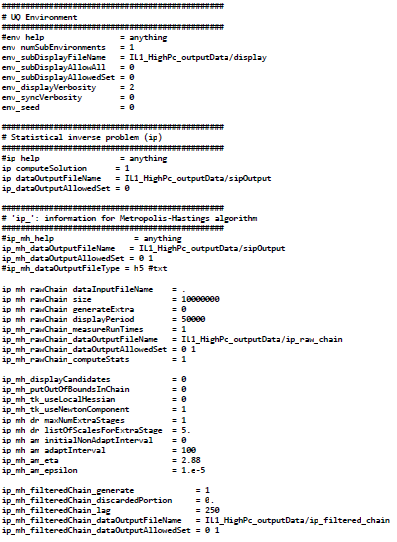
\includegraphics[width=0.75\textwidth]{QUESO_Input_File_Example.png}
\caption{QUESO Input File Example}
\label{QuesoInput}
\end{figure}

\section{Results} \label{results}

The Strand Burner burn rate data was analyzed applying two assumptions. The first assumes 
that all the data could be accurately model using a single Saint Robert's Law. The second 
assumes that two Saint Robert's Law accurately models the data; one for the low pressure 
regime (300 psi � 650 psi) and a second for higher pressure (780 psi � 2000 psi). This 
second assumption is identical to the regression fit performed by the experimenters. It 
also seems reasonable due to the fact that the experimenters reported an intermediate 
pressure regime (650 psi � 780 psi) where the propellant self-extinguished. This behavior 
could indicate that the relative rates between intermediate reactions is changing in each 
pressure regime and may not be well characterized by a single Saint Robert's burn rate law. 
The results based on these assumptions are discussed in of the following sections.

\subsection{Single Burn Rate Law Results} \label{singleRate}

Assuming a single burn rate law could model the observed data resulted in $A$ and $n$ equal 
to 0.9674 and 1.9046, respectively. As can be seen in Figure \ref{SingleBRfig}, this 
results in a burn rate model that fits well with burn rates recorded at pressures $\geq$780 psi.
It does not appear to model the burn rates recorded at pressures $<$780 psi. 
Based on this result, it was conclude that two burn rate laws would model the data better. 
As such, further analysis on this model was not pursued.

\begin{figure}[htb]
\centering
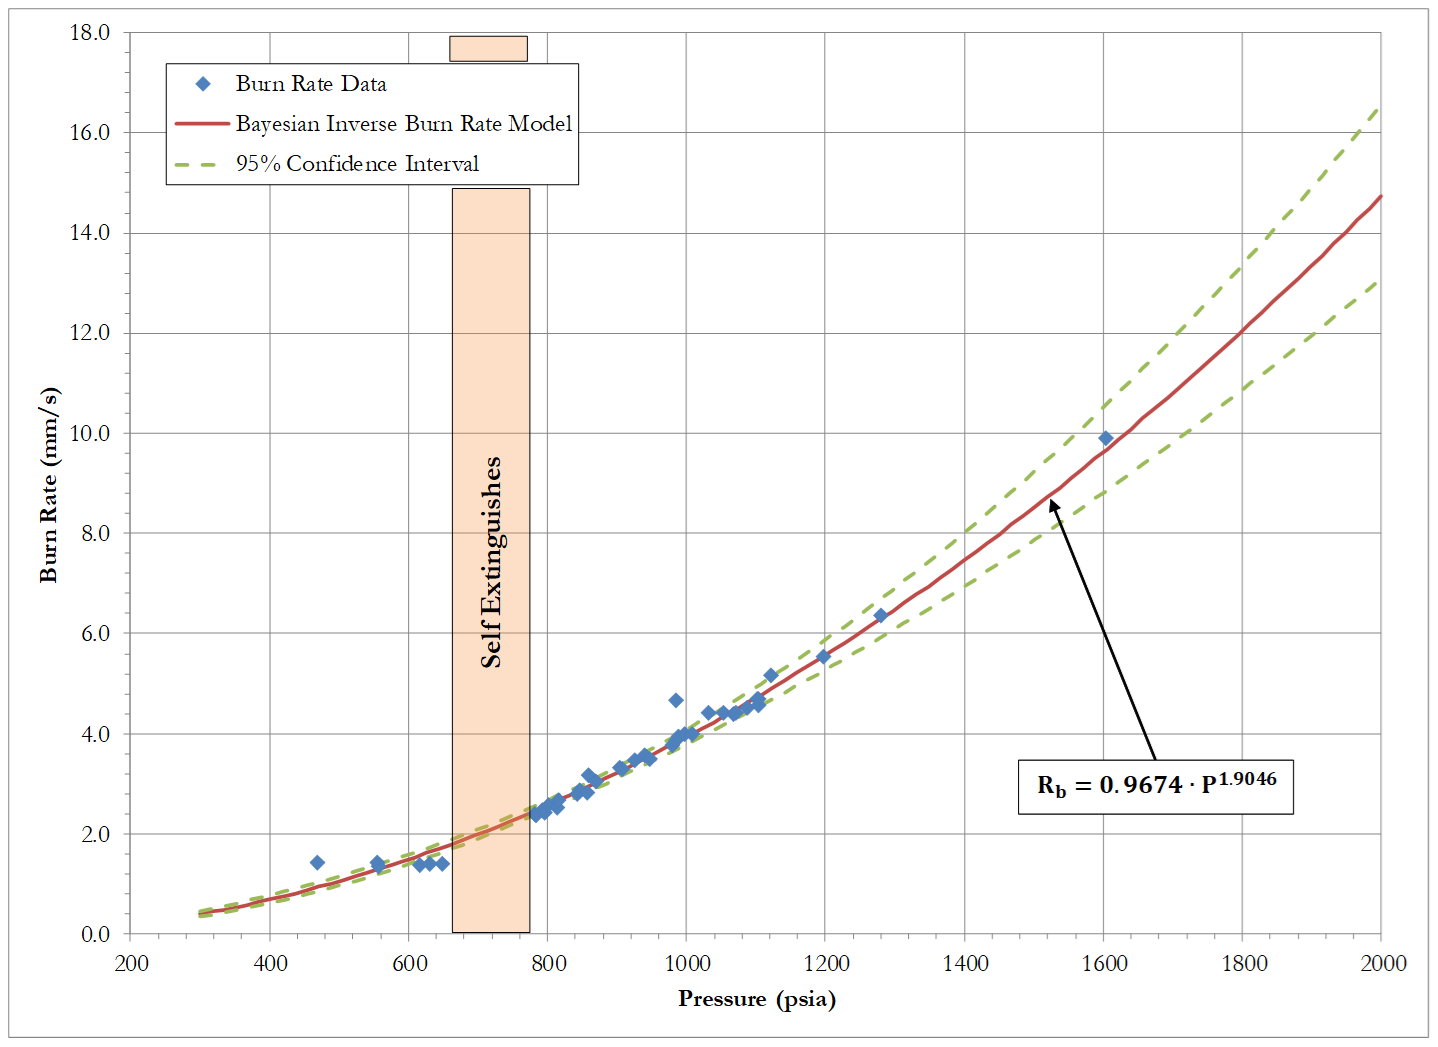
\includegraphics[width=\textwidth]{Single_Burn_Rate_Results.png}
\caption{Single Burn Rate Law Model \& Data Comparison}
\label{SingleBRfig}
\end{figure}

\subsection{Two Burn Rate Law Results} \label{twoBurnRateResults}

Assuming two burn rate laws could model the observed data resulted in the $A$ and $n$ values 
listed in Table \ref{Table:brlpresults} for both pressure regimes. As can be seen from a comparison 
with the experimenters' regression, the current analysis using Bayesian Inversion 
Methods agree well in the high pressure regime. However, the results show that the 
current analysis varies appreciably from the experimenters' regression in the low 
pressure regime. 

\begin{table}
\caption{Burn Rate Law Parameter Results}
\label{Table:brlpresults}
\begin{tabular}{|c|c|c|c|c|}
\hline
Parameter & \multicolumn{2}{|c|}{Bayesian Analysis} & \multicolumn{2}{|c|}{Experimenter's Regression} \\ \cline{2-5}
 & Low Pressure & High Pressure & Low Pressure & High Pressure \\ \hline
$A$ & 1.1880 & $5.1131 \cdot 10^{-6}$ & 1.78 & $5.01 \cdot 10^{-6}$ \\ \hline
$n$ & 0.0215 & 1.9631 & -0.0386 & 1.96 \\
\hline
\end{tabular}
\end{table}

The resulting Bayesian Inversion Method models in both regimes have tight 95\% confidence intervals in 
areas where the data is more concentrated. Figure \ref{DualBRfig} shows the resulting models and 95\% confidence 
intervals compared to the recorded data.

\begin{figure}[htb]
\centering
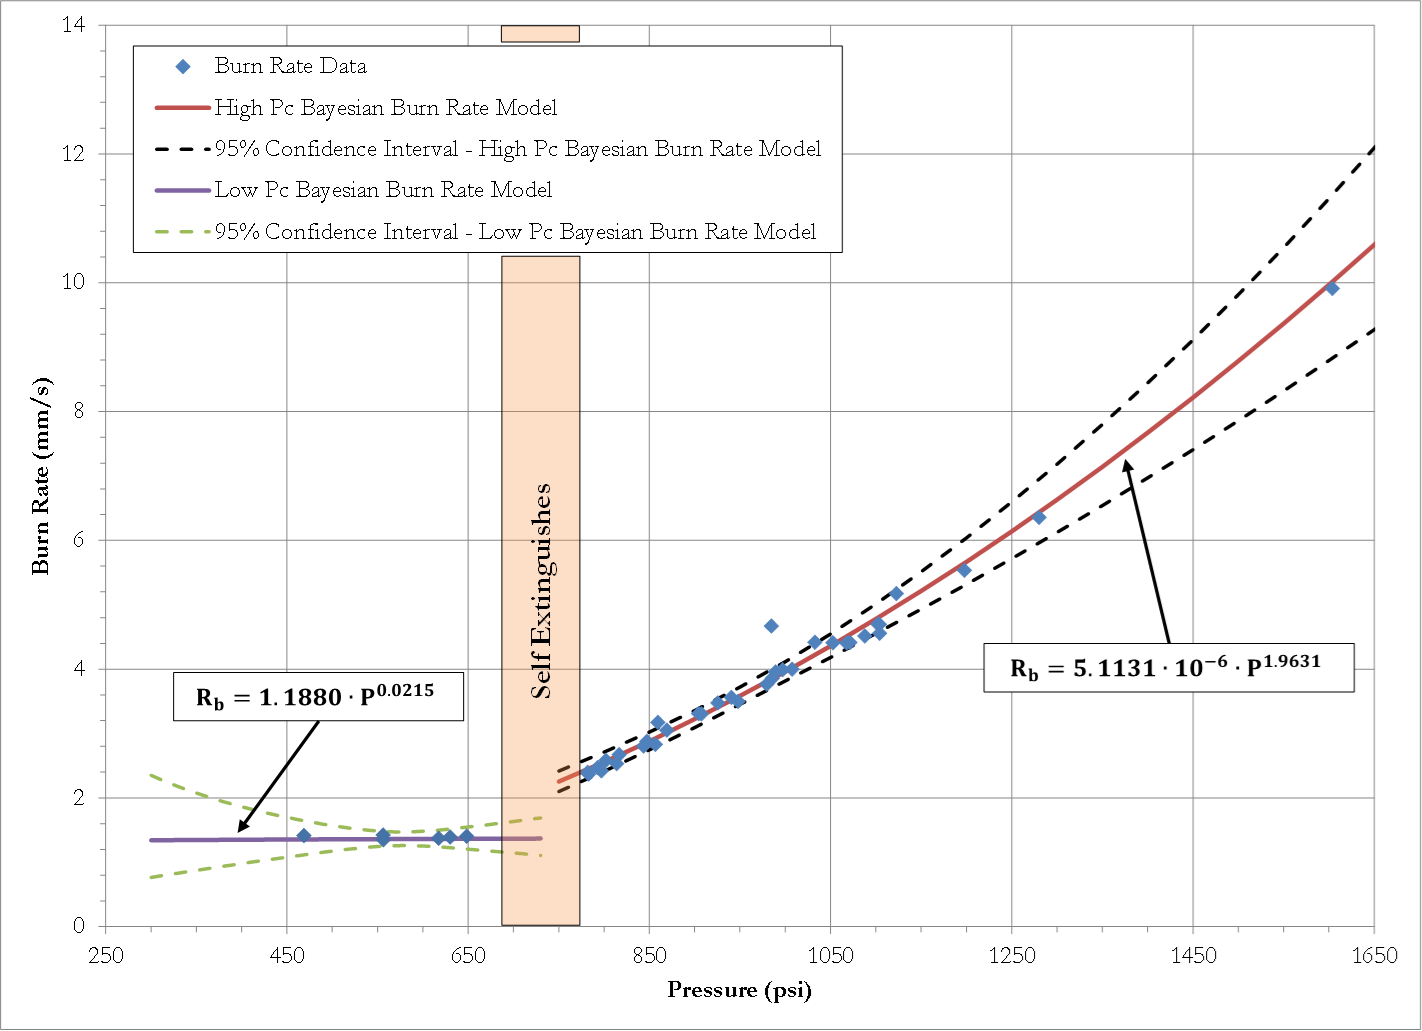
\includegraphics[width=\textwidth]{Dual_Burn_Rate_Results.png}
\caption{Two Burn Rate Law Model \& Data Comparison}
\label{DualBRfig}
\end{figure}

Uncertainty quantification of the burn rate model parameters were investigated using QUESO's Metropolis-Hastings
algorithm. Before providing the resulting Parameter Density Functions (pdf) for each of the parameters in each of 
the models, a plot of the filtered chain is provided in Figures \ref{LPChain} \& \ref{HPChain}. As expected, 
plots which resemble white noise are shown indicating that random samplings of the pdf for each of the parameters
have been successfully taken.

\begin{figure}[htb]
\centering
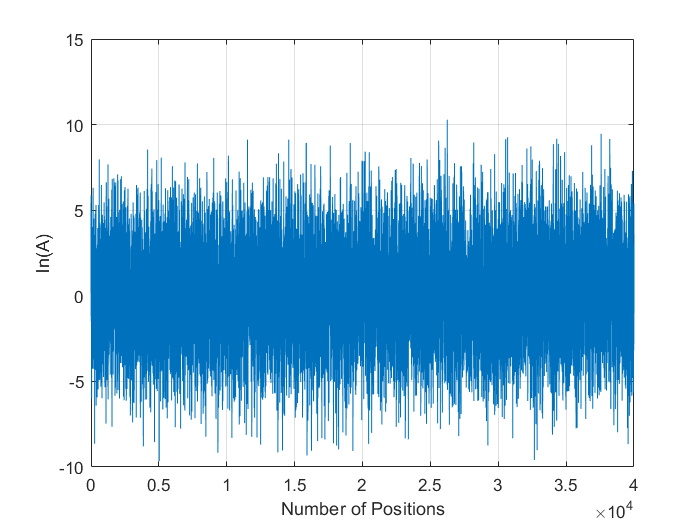
\includegraphics[width=0.48\textwidth]{FilteredChain_lnA_LP.png}
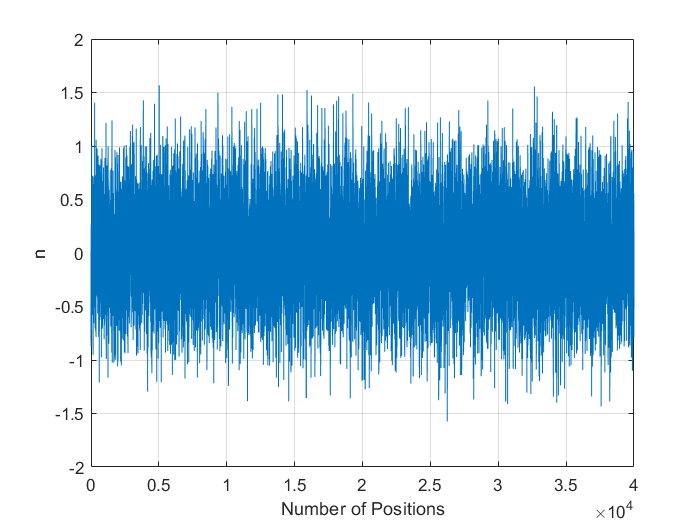
\includegraphics[width=0.48\textwidth]{FilteredChain_n_LP.png}
\caption{Filtered Chain Plot - Low Pressure Model Parameters}
\label{LPChain}
\end{figure}

\begin{figure}[htb]
\centering
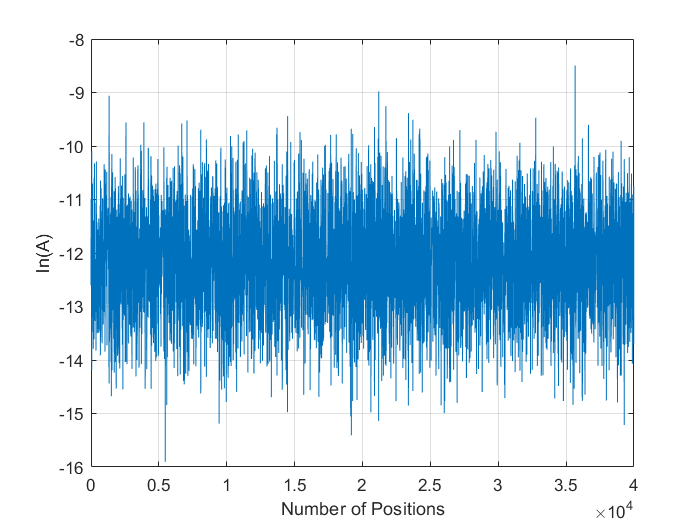
\includegraphics[width=0.48\textwidth]{FilteredChain_lnA_HP.png}
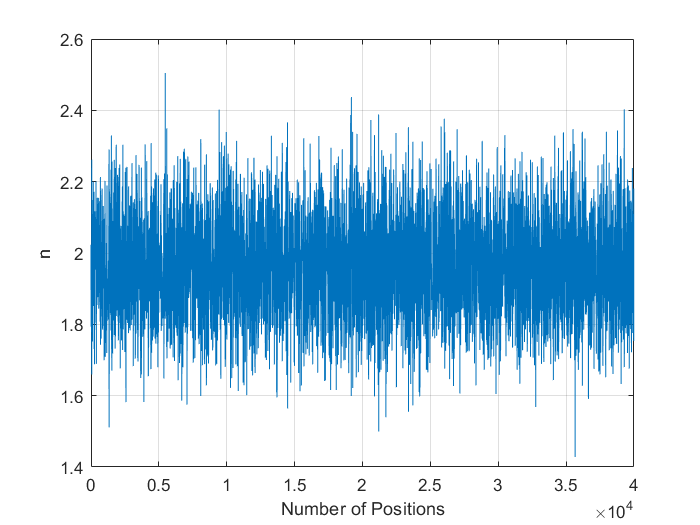
\includegraphics[width=0.48\textwidth]{FilteredChain_n_HP.png}
\caption{Filtered Chain Plot - High Pressure Model Parameters}
\label{HPChain}
\end{figure}

The pdf's for each of the model parameters are provided in Figures \ref{LPpdf} \& \ref{HPpdf}. These figures show that each of 
the parameters' uncertainties have been captured within the -100 to 100 range of the parameter space and show 
a traditional Gaussian profile. The singular peak is reasonably concentrated for each pressure regime model's 
parameter considering the limited number of data points available (9 data points in the low pressure regime, 
35 data points in the high pressure regime).

\begin{figure}[htb]
\centering
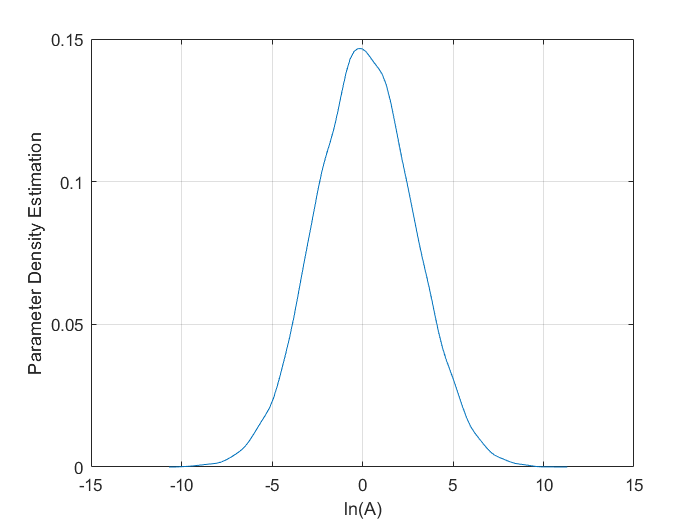
\includegraphics[width=0.48\textwidth]{PDF_lnA_LP.png}
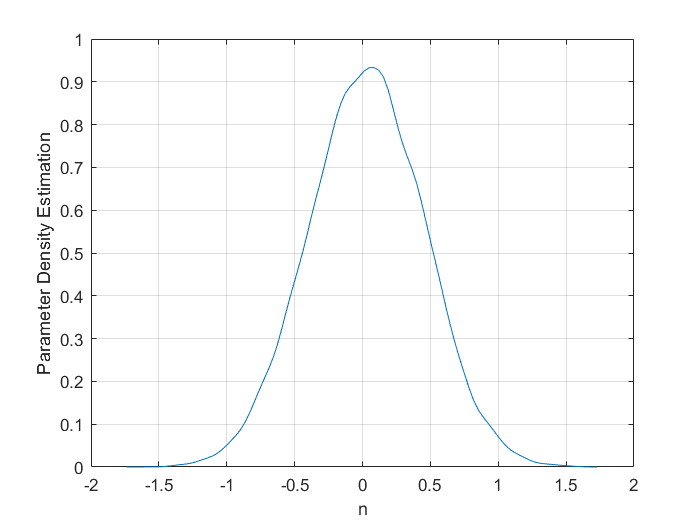
\includegraphics[width=0.48\textwidth]{PDF_n_LP.png}
\caption{Resulting Parameter Density Function - Low Pressure Model Parameters}
\label{LPpdf}
\end{figure}

\begin{figure}[htb]
\centering
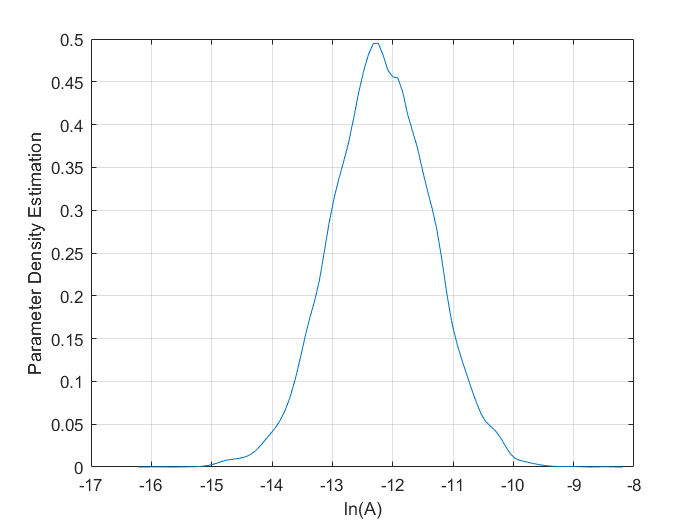
\includegraphics[width=0.48\textwidth]{PDF_lnA_HP.png}
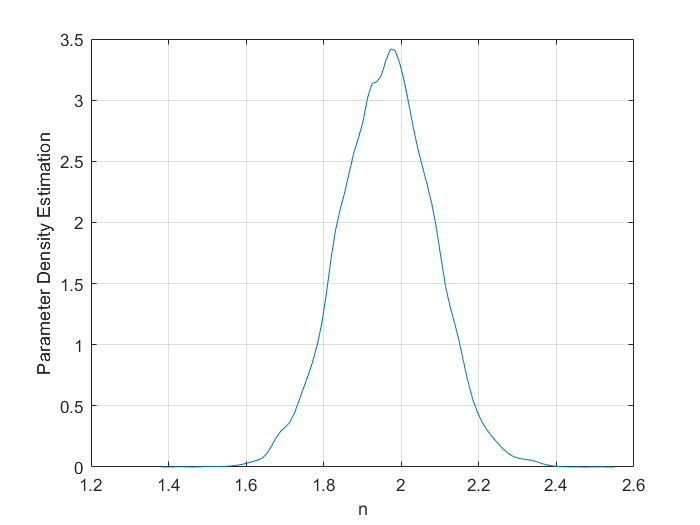
\includegraphics[width=0.48\textwidth]{PDF_n_HP.png}
\caption{Resulting Parameter Density Function - High Pressure Model Parameters}
\label{HPpdf}
\end{figure}

\section{Conclusion} \label{conclusion}

Analysis results show that applying two Saint Robert's Law models, one for low pressure (300 psi � 650 psi) 
and one for high pressure (780 psi � 2000 psi), to predict the burn rate of the candidate ionic liquid propellant 
is more accurate and represents the data better than a single Saint Robert's Law. This is consistent with the 
experimenters' linear regression model of the data. 

A comparison between the experimenters' model and the resulting models presented in this report shows that the 
models agree well for the high pressure regime. The comparison also shows that in the low pressure regime the 
models do not agree well. They particularly diverge in their slope with the experimenters' burn rate model having 
a negative slope and the burn rate model inferred using Bayesian Inversion Methods having a positive slope. The 
expectation is for the burn rate to increase as the pressure increases (i.e. As molecular collision frequencies 
increase, the burn rate of the propellant increases). The Bayesian inferred burn rate model supports this hypothesis. 
On the other hand, there is a marked pressure regime (650 psi $\leq P \leq$ 780 psi) where the propellant self-extinguishes. 
The negative slope put forth by the experimenters' may be an indicator of this behavior. It is possible that the 
experimenters' model and Bayesian Inferred model presented in this report may converge with the availability of additional 
data in the low pressure regime (only 9 data points observed). It is also clear that additional data and/or detailed 
combustion analysis of the propellant is required to better characterize the cause of the propellant's self-extinguishing 
behavior in the intermediate pressure regime.

The results also show that the Bayesian Inversion Methods employed for this analysis has provided additional information 
about the burn rate model which was not provided and/or determined by the experimenters' model. The �for-free� ability 
to determine the 95\% confidence interval from the covariance allows us to a) determine what pressure regimes we should 
collect additional data to improve the models and b) if those experiments were executed, the range over which we would 
most likely expect the burn rate to be. This knowledge would allow the experimenters to determine if the experiment's 
result was expected and may indicate to the experimenters that there was something erroneous with the measurement or 
if the propellant was entering a new burn rate regime from simple inspection of the figures. Both pieces of information 
would allow for better decisions to be made in both determining what to test and assessing the observations in-situ.


\end{document}

